\documentclass[a4paper, 12pt, twoside]{article}


%------------------------------------------------------------------------
%
% Author                :   Lasercata
% Last modification     :   2023.10.02
%
%------------------------------------------------------------------------


%------------------------------------------------------------------------
% This is a LaTeX template, with some useful commands and environments.
%
% Author                :   Lasercata
% Last modification     :   2023.12.18
% Version               :   v6.0.4
%
%------------------------------------------------------------------------


%------ini
\usepackage[utf8]{inputenc}
\usepackage[T1]{fontenc}


%------geometry
\usepackage[textheight=700pt, textwidth=500pt]{geometry}


%------color
\usepackage{xcolor}
\definecolor{ff4500}{HTML}{ff4500}
\definecolor{00f}{HTML}{0000ff}
\definecolor{0ff}{HTML}{00ffff}
\definecolor{656565}{HTML}{656565}

\newcommand{\Emph}{\textcolor{ff4500}}

\newcommand{\strong}[1]{\textcolor{ff4500}{\bf #1}}
\newcommand{\st}{\color{ff4500}\bf}


%------Code highlighting
%---listings
\usepackage{listings}

\definecolor{cbg}{HTML}{272822}
\definecolor{cfg}{HTML}{ececec}
\definecolor{ccomment}{HTML}{686c58}
\definecolor{ckw}{HTML}{f92672}
\definecolor{cstring}{HTML}{e6db72}
\definecolor{cstringlight}{HTML}{98980f}
\definecolor{lightwhite}{HTML}{fafafa}

\lstdefinestyle{DarkCodeStyle}{
    backgroundcolor=\color{cbg},
    commentstyle=\itshape\color{ccomment},
    keywordstyle=\color{ckw},
    numberstyle=\tiny\color{cbg},
    stringstyle=\color{cstring},
    basicstyle=\ttfamily\footnotesize\color{cfg},
    breakatwhitespace=false,
    breaklines=true,
    captionpos=b,
    keepspaces=true,
    numbers=left,
    numbersep=5pt,
    showspaces=false,
    showstringspaces=false,
    showtabs=false,
    tabsize=4,
    xleftmargin=\leftskip
}

\lstdefinestyle{LightCodeStyle}{
    backgroundcolor=\color{lightwhite},
    commentstyle=\itshape\color{ccomment},
    keywordstyle=\color{ckw},
    numberstyle=\tiny\color{cbg},
    stringstyle=\color{cstringlight},
    basicstyle=\ttfamily\footnotesize\color{cbg},
    breakatwhitespace=false,
    breaklines=true,
    captionpos=b,
    keepspaces=true,
    numbers=left,
    numbersep=10pt,
    showspaces=false,
    showstringspaces=false,
    showtabs=false,
    tabsize=4,
    frame=L,
    xleftmargin=\leftskip
}

%\lstset{style=DarkCodeStyle}
\lstset{style=LightCodeStyle}
%Usage : \begin{lstlisting}[language=Caml, xleftmargin=xpt] ... \end{lstlisting}


%---Algorithm
\usepackage[linesnumbered,ruled,vlined]{algorithm2e}
\SetKwInput{KwInput}{Input}
\SetKwInput{KwOutput}{Output}

\SetKwProg{Fn}{Function}{:}{}
\SetKwProg{Proc}{Procedure}{:}{}
\SetKw{KwPrint}{Print}

\newcommand\commfont[1]{\textit{\texttt{\textcolor{656565}{#1}}}}
\SetCommentSty{commfont}
\SetProgSty{texttt}
\SetArgSty{textnormal}
\SetFuncArgSty{textnormal}
%\SetProgArgSty{texttt}

\newenvironment{indalgo}[2][H]{
    \begin{algoBox}
        \begin{algorithm}[#1]
            \caption{#2}
}
{
        \end{algorithm}
    \end{algoBox}
}


%---tcolorbox
\usepackage[many]{tcolorbox}

\DeclareTColorBox{emphBox}{O{black}O{lightwhite}}{
    breakable,
    outer arc=0pt,
    arc=0pt,
    top=0pt,
    toprule=-.5pt,
    right=0pt,
    rightrule=-.5pt,
    bottom=0pt,
    bottomrule=-.5pt,
    colframe=#1,
    colback=#2,
    enlarge left by=10pt,
    width=\linewidth-\leftskip-10pt,
}

\DeclareTColorBox{algoBox}{O{black}O{lightwhite}}{
    breakable,
    arc=0pt,
    top=0pt,
    toprule=-.5pt,
    right=0pt,
    rightrule=-.5pt,
    bottom=0pt,
    bottomrule=-.5pt,
    left=0pt,
    leftrule=-.5pt,
    colframe=#1,
    colback=#2,
    width=\linewidth-\leftskip-10pt,
}


%-------make the table of content clickable
\usepackage{hyperref}
\hypersetup{
    colorlinks,
    citecolor=black,
    filecolor=black,
    linkcolor=black,
    urlcolor=black
}


%------pictures
\usepackage{graphicx}
%\usepackage{wrapfig}

\usepackage{tikz}

\usepackage{float} % For [H] in figure env


%------tabular
%\usepackage{color}
%\usepackage{colortbl}
%\usepackage{multirow}


%------Physics
%---Packages
%\usepackage[version=4]{mhchem} %$\ce{NO4^2-}$

%---Commands
\newcommand{\link}[2]{\mathrm{#1} \! - \! \mathrm{#2}}
\newcommand{\pt}[1]{\cdot 10^{#1}} % Power of ten
\newcommand{\dt}[2][t]{\dfrac{\mathrm d #2}{\mathrm d #1}} % Derivative
\renewcommand{\d}{\mathrm d}

\newcommand{\rot}{\vect{\mathrm{rot}}}
\newcommand{\grad}{\vect{\mathrm{grad}}}
\renewcommand{\div}{\mathrm{div}}
\renewcommand{\j}{\vec\jmath}


%------math
%---Packages
%\usepackage{textcomp}
%\usepackage{amsmath}
\usepackage{amssymb}
\usepackage{mathtools} % For abs
\usepackage{stmaryrd} %for \llbracket and \rrbracket
\usepackage{mathrsfs} %for \mathscr{x} (different from \mathcal{x})
\usepackage{esint} % Better integrals (double, triple, \oiint, ...)

%---Commands
%-Sets
\newcommand{\N}{\mathbb{N}} %set N
\newcommand{\Z}{\mathbb{Z}} %set Z
\newcommand{\Q}{\mathbb{Q}} %set Q
\newcommand{\R}{\mathbb{R}} %set R
\newcommand{\C}{\mathbb{C}} %set C
\newcommand{\U}{\mathbb{U}} %set U
\newcommand{\seg}[2]{\left[ #1\ ;\ #2 \right]}
\newcommand{\nset}[2]{\left\llbracket #1\ ;\ #2 \right\rrbracket}

%-Exponantial / complexs
\newcommand{\e}{\mathrm{e}}
\newcommand{\cj}[1]{\overline{#1}} %overline for the conjugate.

%-Vectors
\newcommand{\vect}{\overrightarrow}
\newcommand{\veco}[3]{\displaystyle \vect{#1}\binom{#2}{#3}} %vector + coord

%-Limits
\newcommand{\lm}[2][{}]{\lim\limits_{\substack{#2 \\ #1}}} %$\lm{x \to a} f$ or $\lm[x < a]{x \to a} f$
\newcommand{\Lm}[3][{}]{\lm[#1]{#2} \left( #3 \right)} %$\Lm{x \to a}{f}$ or $\Lm[x < a]{x \to a}{f}$
\newcommand{\tendsto}[1]{\xrightarrow[#1]{}}

%-Integral
\newcommand{\dint}[4][x]{\displaystyle \int_{#2}^{#3} #4 \mathrm{d} #1} %$\dint{a}{b}{f(x)}$ or $\dint[t]{a}{b}{f(t)}$

%-left right
\newcommand{\lr}[1]{\left( #1 \right)}
\newcommand{\lrb}[1]{\left[ #1 \right]}
\newcommand{\lrbb}[1]{\left\llbracket #1 \right\rrbracket}
\newcommand{\set}[1]{\left\{ #1 \right\}}
\newcommand{\abs}[1]{\left\lvert #1 \right\rvert}
\newcommand{\norm}[1]{\left\lVert #1 \right\rVert}
\newcommand{\ceil}[1]{\left\lceil #1 \right\rceil}
\newcommand{\floor}[1]{\left\lfloor #1 \right\rfloor}
\newcommand{\lrangle}[1]{\left\langle #1 \right\rangle}

%-Boxes
\newcommand{\oboxed}[1]{\textcolor{ff4500}{\boxed{\textcolor{black}{#1}}}} %orange boxed

\newcommand{\rboxed}[1]{\begin{array}{|c} \hline #1 \\ \hline \end{array}} %boxed with right opened
\newcommand{\lboxed}[1]{\begin{array}{c|} \hline #1 \\ \hline \end{array}} %boxed with left opened

\newcommand{\orboxed}[1]{\textcolor{ff4500}{\rboxed{\textcolor{black}{#1}}}} %orange right boxed
\newcommand{\olboxed}[1]{\textcolor{ff4500}{\lboxed{\textcolor{black}{#1}}}} %orange left boxed

%-Others
\newcommand{\para}{/\!/} %//
\newcommand{\ssi}{\ \Leftrightarrow \ }
\newcommand{\eqsys}[2]{\begin{cases} #1 \\ #2 \end{cases}}

\newcommand{\med}[2]{\mathrm{med} \left[ #1\ ;\ #2 \right]}  %$\med{A}{B} -> med[A ; B]$
\newcommand{\Circ}[2]{\mathscr{C}_{#1, #2}}

\renewcommand{\le}{\leqslant}
\renewcommand{\ge}{\geqslant}


%------commands
%---to quote
\newcommand{\simplecit}[1]{\guillemotleft$\;$#1$\;$\guillemotright}
\newcommand{\cit}[1]{\simplecit{\textcolor{656565}{#1}}}
\newcommand{\quo}[1]{\cit{\it #1}}

%---to indent
\newcommand{\ind}[1][20pt]{\advance\leftskip + #1}
\newcommand{\deind}[1][20pt]{\advance\leftskip - #1}

%---to indent a text
\newcommand{\indented}[2][20pt]{\par \ind[#1] #2 \par \deind[#1]}
\newenvironment{indt}[2][20pt]{#2 \par \ind[#1]}{\par \deind} %Titled indented env

%---title
\newcommand{\thetitle}[2]{\begin{center}\textbf{{\LARGE \underline{\Emph{#1} :}} {\Large #2}}\end{center}}

%---Maths environments
%-Proofs
\newenvironment{proof}[1][{}]{\begin{indt}{$\square$ #1}}{$\blacksquare$ \end{indt}}

%-Maths parts (proposition, definition, ...)
\newenvironment{mathpart}[1]{\begin{indt}{\boxed{\text{\textbf{#1}}}}}{\end{indt}}
\newenvironment{mathbox}[1]{\boxed{\text{\textbf{#1}}}\begin{emphBox}}{\end{emphBox}}
\newenvironment{mathul}[1]{\begin{indt}{\underline{\textbf{#1}}}}{\end{indt}}

\newenvironment{theo}{\begin{mathpart}{Théorème}}{\end{mathpart}}
\newenvironment{Theo}{\begin{mathbox}{Théorème}}{\end{mathbox}}

\newenvironment{prop}{\begin{mathpart}{Proposition}}{\end{mathpart}}
\newenvironment{Prop}{\begin{mathbox}{Proposition}}{\end{mathbox}}
\newenvironment{props}{\begin{mathpart}{Propriétés}}{\end{mathpart}}

\newenvironment{defi}{\begin{mathpart}{Définition}}{\end{mathpart}}
\newenvironment{meth}{\begin{mathpart}{Méthode}}{\end{mathpart}}

\newenvironment{Rq}{\begin{mathul}{Remarque :}}{\end{mathul}}
\newenvironment{Rqs}{\begin{mathul}{Remarques :}}{\end{mathul}}

\newenvironment{Ex}{\begin{mathul}{Exemple :}}{\end{mathul}}
\newenvironment{Exs}{\begin{mathul}{Exemples :}}{\end{mathul}}


%------page style
\usepackage{fancyhdr}
\usepackage{lastpage}

\setlength{\headheight}{18pt}
\setlength{\footskip}{50pt}

\pagestyle{fancy}
\fancyhf{}
\fancyhead[LE, RO]{\textit{\textcolor{black}{\today}}}
\fancyhead[RE, LO]{\large{\textsl{\Emph{\texttt{\jobname}}}}}

\fancyfoot[RO, LE]{\textit{\texttt{\textcolor{black}{Page \thepage /}\pageref{LastPage}}}}
% \fancyfoot[LO, RE]{\includegraphics[scale=0.12]{/home/lasercata/Pictures/1.images_profil/logo/mieux/lasercata_logo_fly_fond_blanc.png}}
% \newcommand{\setlogo}{\fancyfoot[LO, RE]{\includegraphics[scale=0.12]{/home/lasercata/Pictures/1.images_profil/logo/mieux/lasercata_logo_fly_fond_blanc.png}}}
\newcommand{\setlogo}[1][/home/lasercata/Pictures/1.images_profil/logo/mieux/lasercata_logo_fly_fond_blanc.png]{\fancyfoot[LO, RE]{\includegraphics[scale=0.12]{#1}}}


%------init lengths
\setlength{\parindent}{0pt} %To avoid using \noindent everywhere.
\setlength{\parskip}{3pt}


\usetikzlibrary{babel}
\usetikzlibrary{shapes.geometric}
\usepackage{circuitikz}


%---------------------------------Begin Document
\begin{document}
    
    %For dark mode :
    % \pagecolor{black}
    % \color{white}
    
    \thetitle{Ti$k$z}{electrical circuits}
    
    %\tableofcontents
    %\newpage

    \begin{circuitikz}
        \draw
        (0,0) to[R=R, o-o] (2,0)
        (4,0) to[vR=vR, o-o] (6,0)
        (0,2) to[transmission line=transmission line, o-o] (2,2)
        (4,2) to[closing switch=closing switch, o-o] (6,2)
        (0,4) to[european current source=european current source, o-o] (2,4)
        (4,4) to[european voltage source=european voltage source, o-o] (6,4)
        (0,6) to[empty diode=empty diode, o-o] (2,6)
        (4,6) to[full led=full led, o-o] (6,6)
        (0,8) to[generic=generic, o-o] (2,8)
        (4,8) to[sinusoidal voltage source=sinusoidal voltage source, o-o] (6,8)
        ;
    \end{circuitikz}

    \begin{circuitikz}
        \draw (0,0)
        to[V,v=$U_q$] (0,2) % The voltage source
        to[nos] (2,2)
        to[generic=$R_1$] (2,0) % The resistor
        to[short] (0,0);
        \draw (2,2)
        to[short] (4,2)
        to[L=$L_1$] (4,0)
        to[short] (2,0);
        \draw (4,2)
        to[short] (6,2)
        to[C=$C_1$] (6,0)
        to[short] (4,0);
   \end{circuitikz}
   
   code :
   
   \begin{lstlisting}[language=tex]
\begin{circuitikz}
    \draw (0,0)
    to[V,v=$U_q$] (0,2) % The voltage source
    to[nos] (2,2)
    to[generic=$R_1$] (2,0) % The resistor
    to[short] (0,0);
    \draw (2,2)
    to[short] (4,2)
    to[L=$L_1$] (4,0)
    to[short] (2,0);
    \draw (4,2)
    to[short] (6,2)
    to[C=$C_1$] (6,0)
    to[short] (4,0);
\end{circuitikz}
   \end{lstlisting}
   
    \begin{circuitikz}
        \draw (0,0) to [capacitor=$C$, o-] (2, 0)
        to [L=$L$] (2, -2)
        to [short, -o] (0, -2);
        \draw (2, -2) to [short] (4, -2)
        to [generic=$R$] (4, 0)
        to [short] (2, 0);
        \draw[->] (0, -1.5) -- node[right] {$u_e$} (0, -.5);
        \draw[->] (4.5, -1.5) -- node[right] {$u_s$} (4.5, -.5);
    \end{circuitikz}
    
    code :
    
    \begin{lstlisting}[language=tex]
\begin{circuitikz}
    \draw (0,0) to [capacitor=$C$, o-] (2, 0)
    to [L=$L$] (2, -2)
    to [short, -o] (0, -2);
    \draw (2, -2) to [short] (4, -2)
    to [generic=$R$] (4, 0)
    to [short] (2, 0);
    \draw[->] (0, -1.5) -- node[right] {$u_e$} (0, -.5);
    \draw[->] (4.5, -1.5) -- node[right] {$u_s$} (4.5, -.5);
\end{circuitikz}
    \end{lstlisting}
    
        \begin{figure}[h!]
        \begin{center}
            \begin{circuitikz}
                \draw (0,0)
                to[V,v=$U_q$] (0,2) % The voltage source
                to[short] (2,2)
                to[R=$R_1$] (2,0) % The resistor
                to[short] (0,0);
            \end{circuitikz}
            \caption{My first circuit.}
        \end{center}
    \end{figure}


    \begin{circuitikz}
        \draw (0, 0) to [lamp] (0, 4)
        ;
    \end{circuitikz}
    
    \begin{circuitikz}
        \draw
        (0,0) to[battery] (0,4)
        to[ammeter] (4,4) 
        to[C] (4,0) -- (3.5,0)
        to[lamp, *-*] (0.5,0) -- (0,0)
        (0.5,0) -- (0.5,-2)
        to[voltmeter] (3.5,-2) -- (3.5,0)
        ;
    \end{circuitikz}


    \begin{center}
        \begin{tikzpicture}
            \draw (0, 0) to [V, v=$\underline E_{\rm g}$] (0, 2)
                to [generic=$R_{\rm g}$, -o] (3, 2);

            \draw (0, 0) to [short, -o] (3, 0);

            \draw[dashed, ff4500] (-1.4, -.5) rectangle (2.5, 2.8);

            \draw (3, 2) to [short, i=$I_{\rm in}$] (4, 2);
            \draw (3, 0) to [short] (11, 0);

            \draw [thick] (4, -.5) rectangle (9, 2.8);
            \node (q) at (4.1, 3.1) {$Q$};

            \draw (11, 2) to [short, i=$I_{\rm out}$] (9, 2);

            \draw (11, 2) to [short, o-] (12, 2)
                to [generic=$\underline Z_{\rm L}$] (12, 0)
                to [short, -o] (11, 0);

            \draw[dashed, blue] (11.5, -.5) rectangle (13, 2.5);

            \draw[->] (3, .3) to node [right] {$V_{\rm in}$} (3, 1.7);
            \draw[->] (11, .3) to node [left] {$V_{\rm out}$} (11, 1.7);

            \node (s) at (0, -1) {source de tension};
            \node (l) at (12, -1) {charge utilisateur};

            \draw[ff4500] (4, 2) to [short] (4.5, 2)
                to [generic=$\underline Z_{\rm in}$, color=ff4500] (4.5, 0);

            \draw[blue] (7.7, 0) to [V, v=$\underline A_{V_0} \cdot V_{\rm in}$, color=blue] (7.7, 2)
                to [generic=$\underline Z_{\rm out}$, color=blue] (9, 2);
        \end{tikzpicture}
    \end{center}


    \begin{center}
        \begin{tikzpicture}
            \draw (0, 0) node [above] {$A_1$} to [generic=$\underline Y_1$, o-] (2, 0)
                to [short, -o] (3, 0)
                to (4, 0) node [op amp, anchor=-] (AO1) {\texttt{AOIL 1}};

            % \draw (AO1.+) to (3, -2);
            \draw (AO1.out) to [short, -o] (8, -.5) node [above] {$A_2$};

            \draw (6.5, -.5) to [short, *-] (6.5, 1.5)
                to [generic=$\underline Y_2$] (3, 1.5)
                to [short, -*] (3, 0) node [above left] {$B_1$};

            \draw (AO1.+) to [short, -*] (4, -2);
            \node at (5, -2) [eground] {};

            % \node at (0, -2) [eground] {};
            \draw[->] (0, -1.7) to node [right] {$\underline s_1$} (0, -.3);

            % \node at (8, -2) [eground] {};
            \draw[->] (8, -1.7) to node [right] {$\underline s_2$} (8, -.7);

            \draw[->] (4, -.7) to node [left] {$\varepsilon_1$} (4, -.3);
            \draw[->] (3, -1.7) to node [left] {$v_1^-$} (3, -.3);

            \draw (0, -2) to [short, o-o] (8, -2);
        \end{tikzpicture}
    \end{center}


    \begin{center}
        \begin{tikzpicture}
            % \draw (0, 0) node [above] {$B_1$} to [short, *-] (-2, 0)
            %     to [generic={$R_2$}] (-2, -2)
            %     to [european voltage source={$s_1$}] (-2, -4);

            \draw (-2, -4) [european voltage source={$\underline s_1$}, *-] to (-2, -2);
            \draw (-2, -2) to [generic={$\underline Y_1$}] (-2, 0)
                to [short, -*] (0, 0) node [above] {$B_1$};

            \draw (2, -4) [european voltage source={$\underline s_2$}, *-] to (2, -2);
            \draw (2, -2) to [generic={$\underline Y_2$}] (2, 0)
                to [short, -*] (0, 0) node [above] {$B_1$};

            \draw (-2, -4) to [short] (2, -4);
            \node at (0, -4) [eground] {};

            \draw[->] (0, -3.7) to node [left] {$v_1^- = 0$} (0, -.3);
        \end{tikzpicture}
    \end{center}
    
    
    
\end{document}
%--------------------------------------------End
